% Options for packages loaded elsewhere
\PassOptionsToPackage{unicode}{hyperref}
\PassOptionsToPackage{hyphens}{url}
%
\documentclass[
]{book}
\usepackage{amsmath,amssymb}
\usepackage{lmodern}
\usepackage{ifxetex,ifluatex}
\ifnum 0\ifxetex 1\fi\ifluatex 1\fi=0 % if pdftex
  \usepackage[T1]{fontenc}
  \usepackage[utf8]{inputenc}
  \usepackage{textcomp} % provide euro and other symbols
\else % if luatex or xetex
  \usepackage{unicode-math}
  \defaultfontfeatures{Scale=MatchLowercase}
  \defaultfontfeatures[\rmfamily]{Ligatures=TeX,Scale=1}
\fi
% Use upquote if available, for straight quotes in verbatim environments
\IfFileExists{upquote.sty}{\usepackage{upquote}}{}
\IfFileExists{microtype.sty}{% use microtype if available
  \usepackage[]{microtype}
  \UseMicrotypeSet[protrusion]{basicmath} % disable protrusion for tt fonts
}{}
\makeatletter
\@ifundefined{KOMAClassName}{% if non-KOMA class
  \IfFileExists{parskip.sty}{%
    \usepackage{parskip}
  }{% else
    \setlength{\parindent}{0pt}
    \setlength{\parskip}{6pt plus 2pt minus 1pt}}
}{% if KOMA class
  \KOMAoptions{parskip=half}}
\makeatother
\usepackage{xcolor}
\IfFileExists{xurl.sty}{\usepackage{xurl}}{} % add URL line breaks if available
\IfFileExists{bookmark.sty}{\usepackage{bookmark}}{\usepackage{hyperref}}
\hypersetup{
  pdftitle={Data Science for Biologists - 5023Y},
  pdfauthor={Philip Leftwich},
  hidelinks,
  pdfcreator={LaTeX via pandoc}}
\urlstyle{same} % disable monospaced font for URLs
\usepackage{color}
\usepackage{fancyvrb}
\newcommand{\VerbBar}{|}
\newcommand{\VERB}{\Verb[commandchars=\\\{\}]}
\DefineVerbatimEnvironment{Highlighting}{Verbatim}{commandchars=\\\{\}}
% Add ',fontsize=\small' for more characters per line
\usepackage{framed}
\definecolor{shadecolor}{RGB}{248,248,248}
\newenvironment{Shaded}{\begin{snugshade}}{\end{snugshade}}
\newcommand{\AlertTok}[1]{\textcolor[rgb]{0.94,0.16,0.16}{#1}}
\newcommand{\AnnotationTok}[1]{\textcolor[rgb]{0.56,0.35,0.01}{\textbf{\textit{#1}}}}
\newcommand{\AttributeTok}[1]{\textcolor[rgb]{0.77,0.63,0.00}{#1}}
\newcommand{\BaseNTok}[1]{\textcolor[rgb]{0.00,0.00,0.81}{#1}}
\newcommand{\BuiltInTok}[1]{#1}
\newcommand{\CharTok}[1]{\textcolor[rgb]{0.31,0.60,0.02}{#1}}
\newcommand{\CommentTok}[1]{\textcolor[rgb]{0.56,0.35,0.01}{\textit{#1}}}
\newcommand{\CommentVarTok}[1]{\textcolor[rgb]{0.56,0.35,0.01}{\textbf{\textit{#1}}}}
\newcommand{\ConstantTok}[1]{\textcolor[rgb]{0.00,0.00,0.00}{#1}}
\newcommand{\ControlFlowTok}[1]{\textcolor[rgb]{0.13,0.29,0.53}{\textbf{#1}}}
\newcommand{\DataTypeTok}[1]{\textcolor[rgb]{0.13,0.29,0.53}{#1}}
\newcommand{\DecValTok}[1]{\textcolor[rgb]{0.00,0.00,0.81}{#1}}
\newcommand{\DocumentationTok}[1]{\textcolor[rgb]{0.56,0.35,0.01}{\textbf{\textit{#1}}}}
\newcommand{\ErrorTok}[1]{\textcolor[rgb]{0.64,0.00,0.00}{\textbf{#1}}}
\newcommand{\ExtensionTok}[1]{#1}
\newcommand{\FloatTok}[1]{\textcolor[rgb]{0.00,0.00,0.81}{#1}}
\newcommand{\FunctionTok}[1]{\textcolor[rgb]{0.00,0.00,0.00}{#1}}
\newcommand{\ImportTok}[1]{#1}
\newcommand{\InformationTok}[1]{\textcolor[rgb]{0.56,0.35,0.01}{\textbf{\textit{#1}}}}
\newcommand{\KeywordTok}[1]{\textcolor[rgb]{0.13,0.29,0.53}{\textbf{#1}}}
\newcommand{\NormalTok}[1]{#1}
\newcommand{\OperatorTok}[1]{\textcolor[rgb]{0.81,0.36,0.00}{\textbf{#1}}}
\newcommand{\OtherTok}[1]{\textcolor[rgb]{0.56,0.35,0.01}{#1}}
\newcommand{\PreprocessorTok}[1]{\textcolor[rgb]{0.56,0.35,0.01}{\textit{#1}}}
\newcommand{\RegionMarkerTok}[1]{#1}
\newcommand{\SpecialCharTok}[1]{\textcolor[rgb]{0.00,0.00,0.00}{#1}}
\newcommand{\SpecialStringTok}[1]{\textcolor[rgb]{0.31,0.60,0.02}{#1}}
\newcommand{\StringTok}[1]{\textcolor[rgb]{0.31,0.60,0.02}{#1}}
\newcommand{\VariableTok}[1]{\textcolor[rgb]{0.00,0.00,0.00}{#1}}
\newcommand{\VerbatimStringTok}[1]{\textcolor[rgb]{0.31,0.60,0.02}{#1}}
\newcommand{\WarningTok}[1]{\textcolor[rgb]{0.56,0.35,0.01}{\textbf{\textit{#1}}}}
\usepackage{longtable,booktabs,array}
\usepackage{calc} % for calculating minipage widths
% Correct order of tables after \paragraph or \subparagraph
\usepackage{etoolbox}
\makeatletter
\patchcmd\longtable{\par}{\if@noskipsec\mbox{}\fi\par}{}{}
\makeatother
% Allow footnotes in longtable head/foot
\IfFileExists{footnotehyper.sty}{\usepackage{footnotehyper}}{\usepackage{footnote}}
\makesavenoteenv{longtable}
\usepackage{graphicx}
\makeatletter
\def\maxwidth{\ifdim\Gin@nat@width>\linewidth\linewidth\else\Gin@nat@width\fi}
\def\maxheight{\ifdim\Gin@nat@height>\textheight\textheight\else\Gin@nat@height\fi}
\makeatother
% Scale images if necessary, so that they will not overflow the page
% margins by default, and it is still possible to overwrite the defaults
% using explicit options in \includegraphics[width, height, ...]{}
\setkeys{Gin}{width=\maxwidth,height=\maxheight,keepaspectratio}
% Set default figure placement to htbp
\makeatletter
\def\fps@figure{htbp}
\makeatother
\setlength{\emergencystretch}{3em} % prevent overfull lines
\providecommand{\tightlist}{%
  \setlength{\itemsep}{0pt}\setlength{\parskip}{0pt}}
\setcounter{secnumdepth}{5}
\usepackage{booktabs}
\usepackage{amsthm}
\makeatletter

\newenvironment{kframe}{%
\medskip{}
\setlength{\fboxsep}{.8em}
 \def\at@end@of@kframe{}%
 \ifinner\ifhmode%
  \def\at@end@of@kframe{\end{minipage}}%
  \begin{minipage}{\columnwidth}%
 \fi\fi%
 \def\FrameCommand##1{\hskip\@totalleftmargin \hskip-\fboxsep
 \colorbox{shadecolor}{##1}\hskip-\fboxsep
     % There is no \\@totalrightmargin, so:
     \hskip-\linewidth \hskip-\@totalleftmargin \hskip\columnwidth}%
 \MakeFramed {\advance\hsize-\width
   \@totalleftmargin\z@ \linewidth\hsize
   \@setminipage}}%
 {\par\unskip\endMakeFramed%
 \at@end@of@kframe}
\makeatother

\makeatletter
\@ifundefined{Shaded}{
}{\renewenvironment{Shaded}{\begin{kframe}}{\end{kframe}}}
\makeatother

\newenvironment{block}[1]
  {
  \begin{itemize}
  \renewcommand{\labelitemi}{
    \raisebox{-.7\height}[0pt][0pt]{
      {\setkeys{Gin}{width=3em,keepaspectratio}\includegraphics{images/#1}}
    }
  }
  \setlength{\fboxsep}{1em}
  \begin{kframe}
  \item
  }
  {
  \end{kframe}
  \end{itemize}
  }
\newenvironment{rmdnote}
  {\begin{block}{note}}
  {\end{block}}
\newenvironment{rmdtip}
  {\begin{block}{tip}}
  {\end{block}}
\newenvironment{rmdwarning}
  {\begin{block}{warning}}
  {\end{block}}
  
\def\thm@space@setup{%
  \thm@preskip=8pt plus 2pt minus 4pt
  \thm@postskip=\thm@preskip
}
\makeatother
\usepackage{booktabs}
\usepackage{longtable}
\usepackage{array}
\usepackage{multirow}
\usepackage{wrapfig}
\usepackage{float}
\usepackage{colortbl}
\usepackage{pdflscape}
\usepackage{tabu}
\usepackage{threeparttable}
\usepackage{threeparttablex}
\usepackage[normalem]{ulem}
\usepackage{makecell}
\usepackage{xcolor}
\ifluatex
  \usepackage{selnolig}  % disable illegal ligatures
\fi
\usepackage[]{natbib}
\bibliographystyle{apalike}

\title{Data Science for Biologists - 5023Y}
\author{Philip Leftwich}
\date{2021-09-26}

\begin{document}
\maketitle

{
\setcounter{tocdepth}{1}
\tableofcontents
}
\hypertarget{introduction}{%
\chapter{Introduction}\label{introduction}}

\hypertarget{approach-and-style}{%
\section{Approach and style}\label{approach-and-style}}

This book is designed to accompany the module BIO-5023Y for those new to R looking for best practices and tips. So it must be both accessible and succinct. The approach here is to provide just enough text explanation that someone very new to R can apply the code and follow what the code is doing. It is not a comprehensive textbook.

A few other points:

This is a code reference book accompanied by relatively brief examples - not a thorough textbook on R or data science

This is intended to be a living document - optimal R packages for a given task change often and we welcome discussion about which to emphasize in this handbook

Top tips for the course:

\textbf{DON'T} worry if you don't understand everything

\textbf{DO} ask lots of questions!

\citet{R-bookdown}

\hypertarget{Unix}{%
\chapter{Unix}\label{Unix}}

Unix is very likely the most fundamental skillset we can develop for bioinformatics (and much more than bioinformatics). Many of the most common and powerful bioinformatics approaches happen in this text-based environment, and having a solid foundation here can make everything we're trying to learn and do much easier. This is a short introductory tutorial to help us get from being completely new to Unix up to being friendly with it 🙂

\hypertarget{what-is-unixlinux}{%
\section{What is Unix/Linux?}\label{what-is-unixlinux}}

UNIX is a computer operating system. It was first developed in 1969 at Bell Labs. Unix is written in the programming language \texttt{C}.

Unix is proprietary software, whereas Linux is \emph{basically} free and open-source Unix.

The Linux Operating System is highly flexible, free, open-source (like R) and uses very little RAM to run (Unlike Windows OS) - as such you find most supercomputers run on Linux. Operationally Linux is almost identical to Unix, and so we often refer to it under the umbrella term of ``unix-Like'' systems.

\hypertarget{some-terms}{%
\subsection{Some terms}\label{some-terms}}

Here are some terms worth knowing, don't worry about memorising them, it can just be useful to have these to refer to in the future.

\begin{longtable}{ll}
\toprule
\textbf{Term} & \textbf{What it is}\\
\midrule
shell & what we use to talk to the computer; anything where you are pointing and clicking with a mouse is a Graphical User Interface (GUI) shell; something with text only is a Command Line Interface (CLI) shell\\
command line & a text-based environment capable of taking input and providing output\\
Terminal & A program that runs a shell\\
Unix & a family of operating systems (we also use the term “Unix-like” because one of the most popular operating systems derived from Unix is specifically named as not being Unix)\\
Linux & a "Unix-like" OS\\
\addlinespace
bash & the most common programming language used at a Unix command-line\\
flag & a way to set options for a function, a specific type of argument usually preceded by a -\\
\bottomrule
\end{longtable}

\begin{quote}
\textbf{Note}

You should be very familiar with using a GUI (RStudio), but remember we have spent a lot of time working with files and directories using the the command line (CLI) in R. This is useful practice, because most supercomputers lack a GUI, you must work entirely using the command line.
\end{quote}

\hypertarget{why-learn-unix}{%
\section{Why Learn Unix?}\label{why-learn-unix}}

Most sequencing data files are large, and require a lot of RAM to process. As a result most of the work Bioinformaticians do is not hosted on their own computers, instead they ``remote-connect'' to high performance supercomputers or cluster computers. Almost all of these high performance computers use ``Unix-like'' operatings systems, the most common of which is Linux.

As stated above Linux is free (so no expensive licenses), open-source so lots of developers, its also well known for being stable, secure, reliable and efficient.

You already have some experience with using a Linux OS - every time you log into RStudio Cloud you are connecting to a supercomputer that runs on Linux. Normally we do not interact directly with the OS, instead we use R and RStudio directly.

But when you click on the RStudio Terminal it provides direct access to a command-line where we can execute commands and functions directly in Linux.

This allows us to start using programs other than R, and potentially use multiple programs \& programming languages to work together.

\begin{quote}
\textbf{Note}

This series of practicals is designed for you to have a first introduction to Bioinformatics, it's about exposure, not memorising or mastering anything. Don't worry about the details!
\end{quote}

\hypertarget{getting-started}{%
\section{Getting started}\label{getting-started}}

Before we get started we need a terminal to work in.

\begin{itemize}
\item
  Open the Bioinformatics RStudio Cloud Project in the 5023Y workspace
\item
  Click on the \texttt{Terminal} tab next to \texttt{Console} in the bottom-left pane of the RStudio GUI, this opens a command-line \emph{Shell}
\end{itemize}

\begin{figure}

{\centering 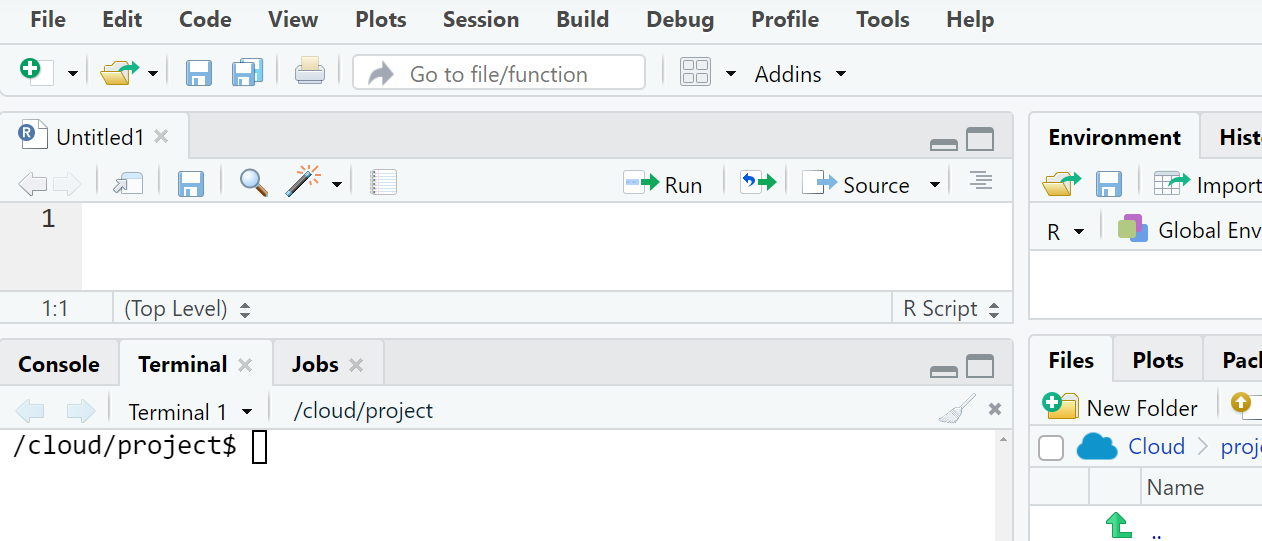
\includegraphics[width=0.8\linewidth]{images/terminal} 

}

\caption{Here is an example of the Terminal tab, right next to the R console}\label{fig:unnamed-chunk-4}
\end{figure}

\begin{itemize}
\item
  This is our ``command line'' where we will be typing all of our commands. We type our commands in \texttt{bash}
\item
  The \$ is where you start typing from, left of this it tells you what folder you are currently in (\texttt{working\ directory})
\item
  If you need to, you can exit the Terminal and start a new session easily with options in RStudio
\end{itemize}

\hypertarget{a-few-foundational-rules}{%
\section{A few foundational rules}\label{a-few-foundational-rules}}

\begin{itemize}
\item
  Just like in R spaces are special, spaces break things apart, as a rule it is therefore better to have functions and file names with dashes (-) or underscores (\_) - e.g.~``draft\_v3.txt'' is preferred to ``draft v3.txt''.
\item
  The general syntax on the command line is: \texttt{command\ argument}. Again this is very similar to R except we don't use brackets e.g.~in R we are used to \texttt{command(argument)}
\item
  Arguments can be \textbf{optional} e.g.~if their is a default argument you may not have to write anything. Some functions \emph{require} that arguments are specified. Again this is just like R.
\end{itemize}

\hypertarget{lets-get-started}{%
\section{Let's get started}\label{lets-get-started}}

We will perform a very simple function and get a flavour of the similarities and differences to working in \texttt{R}.

\texttt{date} is a command that prints out the date and time. Copy and paste this command into your terminal

\begin{Shaded}
\begin{Highlighting}[]
    \FunctionTok{date}
\end{Highlighting}
\end{Shaded}

This prints out the date/time in UTC

More information on using the date function (here){[}\url{https://www.geeksforgeeks.org/date-command-linux-examples/}{]}

We can also ask for the output for a particular timezone using the \texttt{TZ} function and \texttt{date}

\begin{Shaded}
\begin{Highlighting}[]
    \VariableTok{TZ=}\NormalTok{Europe/London }\FunctionTok{date}
\end{Highlighting}
\end{Shaded}

Or we can ask the computer what the date will be next Tuesday\ldots{}

\begin{Shaded}
\begin{Highlighting}[]
    \FunctionTok{date} \AttributeTok{{-}{-}date}\OperatorTok{=}\StringTok{"next tue"}
\end{Highlighting}
\end{Shaded}

\hypertarget{downloading-data}{%
\subsection{Downloading data}\label{downloading-data}}

We will start by typing in an instruction to download data from an online data repository, unpack the contents and inspect it:

\begin{itemize}
\item
  curl is a command line tool for transferring data to and from the server here we will use this to download data from an online repository.
\item
  tar will \emph{unpack} the data from a compressed file format
\item
  cd change the directory so we \emph{land} in the new folder we have made
\end{itemize}

\begin{Shaded}
\begin{Highlighting}[]
    \ExtensionTok{curl} \AttributeTok{{-}L} \AttributeTok{{-}o}\NormalTok{ unix\_intro.tar.gz https://ndownloader.figshare.com/files/15573746}
    \FunctionTok{tar} \AttributeTok{{-}xzvf}\NormalTok{ unix\_intro.tar.gz }\KeywordTok{\&\&} \FunctionTok{rm}\NormalTok{ unix\_intro.tar.gz}
    \BuiltInTok{cd}\NormalTok{ unix\_intro}
\end{Highlighting}
\end{Shaded}

\begin{rmdwarning}
Check each command line has run, in the example above you might find
that the first two lines run, to download and unpack data, while the
last line to change directory doesn't run until you hit enter
\end{rmdwarning}

\hypertarget{more-functions}{%
\subsection{More functions}\label{more-functions}}

Unlike date, most commands require arguments and won't work without them. head is a command that prints the first lines of a file, so it requires us to provide the file we want it to act on:

\begin{Shaded}
\begin{Highlighting}[]
    \FunctionTok{head}\NormalTok{ example.txt}
\end{Highlighting}
\end{Shaded}

Here ``example.txt'' is the required argument, and in this case it is also what's known as a positional argument. Whether things need to be provided as positional arguments or not depends on how the command or program we are using was written.

Sometimes we need to specify the input file by putting something in front of it (e.g.~some commands will use the -i flag, but it's often other things as well).

\textbf{Q. What's in the text file? - Click here for Answer}

\emph{Pretty boring, each line contains the text ``This is line'' followed by the line number e.g.}

\emph{- This is line 1}

\emph{- This is line 2}

\emph{etc.}

There are also optional arguments for the head command. The default for head is to print the first 10 lines of a file. We can change that by specifying the -n flag, followed by how many lines we want:

\begin{Shaded}
\begin{Highlighting}[]
    \FunctionTok{head} \AttributeTok{{-}n}\NormalTok{ 5 example.txt}
\end{Highlighting}
\end{Shaded}

How would we know we needed the -n flag for that? There are a few ways to find out. Many standard Unix commands and other programs will have built-in help menus that we can access by providing --help as the only argument:

\begin{Shaded}
\begin{Highlighting}[]
    \FunctionTok{head} \AttributeTok{{-}{-}help}
\end{Highlighting}
\end{Shaded}

Again this is very similar to the logic in which R commands are strucutred e.g.~\texttt{??ggplot()} The synatx is similar even if the specific icons or arguments are different.

Remember just like with R, one of your best friends is Google! As you get familiar with any language or OS we might remember a few flags or specific options, but searching for options and details when needed is definitely the norm!

\hypertarget{unix-file-structure}{%
\section{Unix File Structure}\label{unix-file-structure}}

There are two special locations in all Unix-based systems: the ``root'' location and the current user's ``home'' location. ``Root'' is where the address system of the computer starts; ``home'' is usally where the current user's location starts.

Just to be awkward RStudio Cloud actually has us working in a different location ``Cloud'', which is underneath Root but separate to home which would be in the ``Users'' folder.

\begin{center}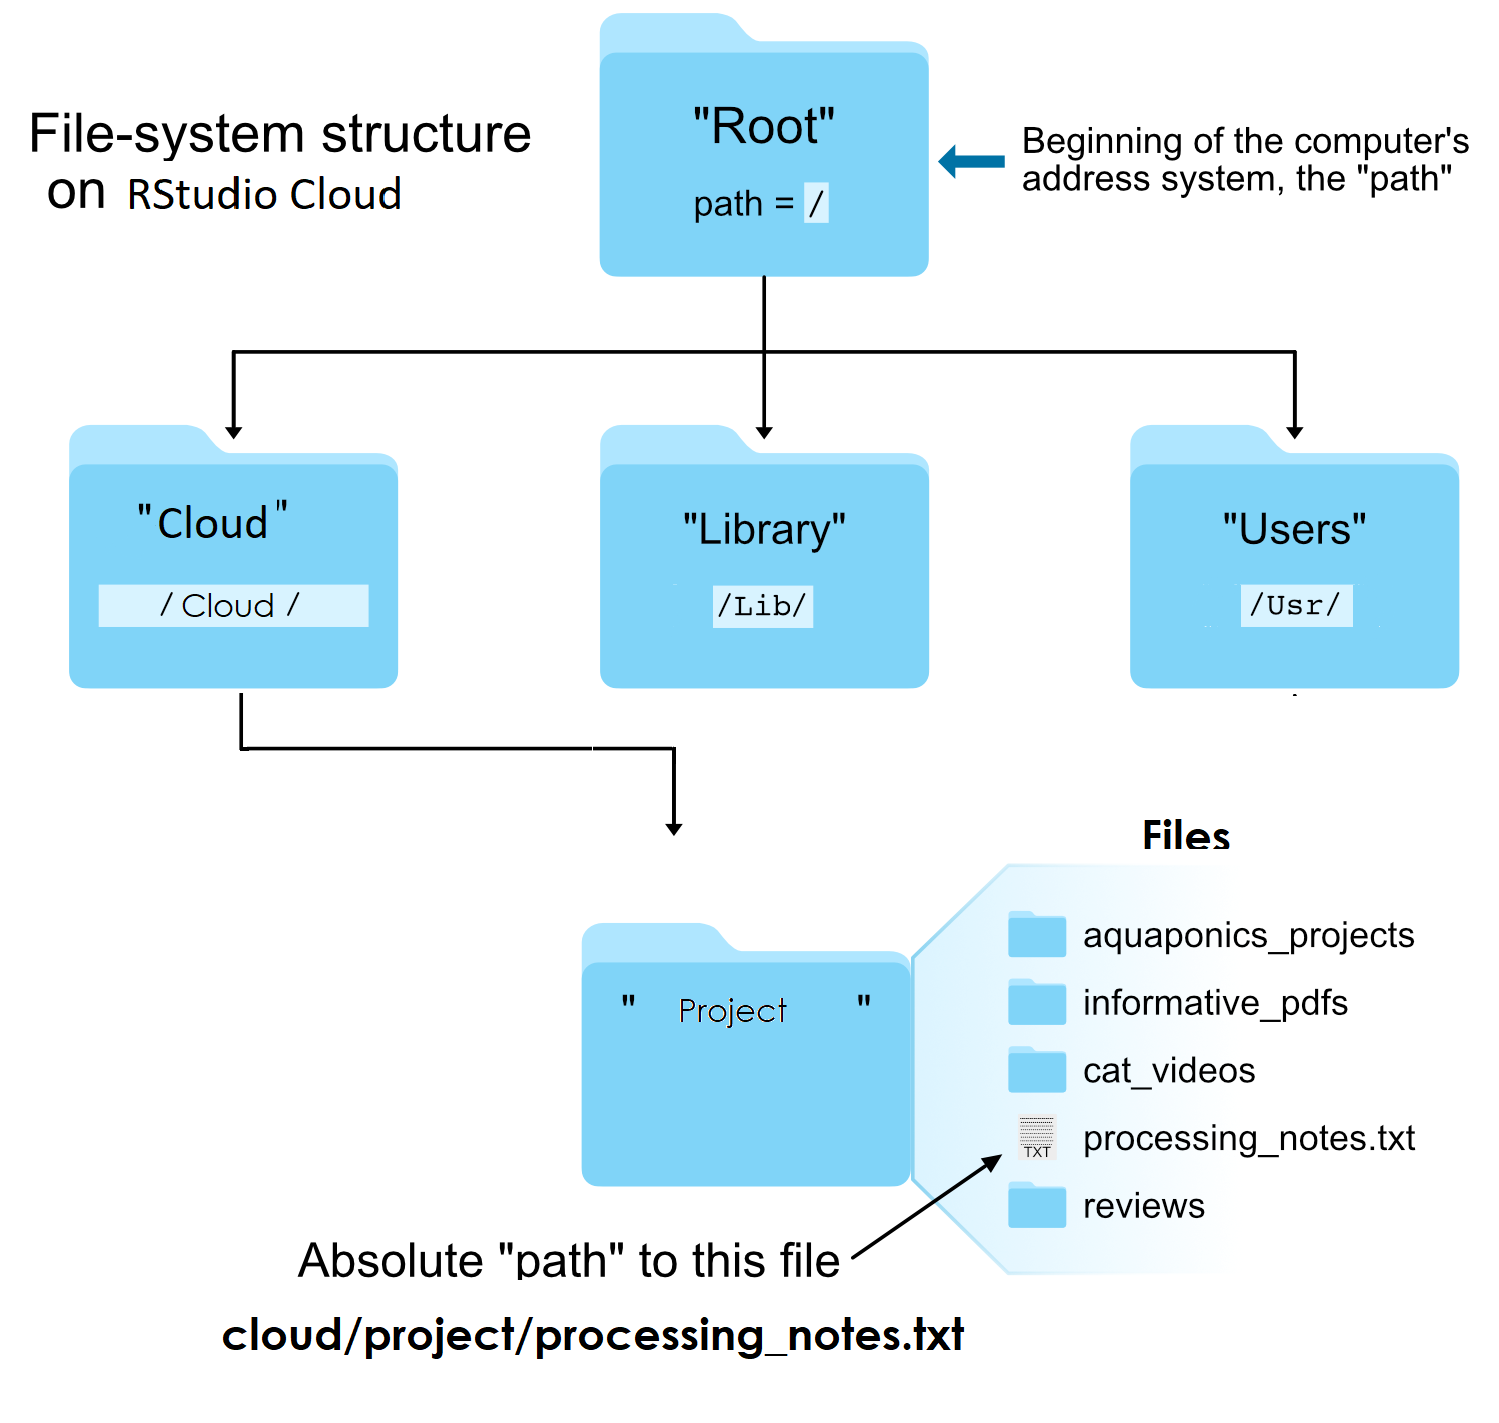
\includegraphics[width=0.8\linewidth]{images/file_system_structure} \end{center}

We tell the command line where files and directories are located by providing their address, their ``path''. If we use the pwd command (for print working directory), we can find out what the path is for the directory we are sitting in.

\begin{Shaded}
\begin{Highlighting}[]
    \BuiltInTok{pwd}
\end{Highlighting}
\end{Shaded}

And if we use the ls command (for list), we can see what directories and files are in the current directory we are sitting in.

\begin{Shaded}
\begin{Highlighting}[]
    \FunctionTok{ls}
\end{Highlighting}
\end{Shaded}

\begin{quote}
\textbf{Note}

Why is it important to know this? Usually when you are working on a Unix-like environment there is no GUI (nice-click and point interface), all commands have to be submitted through the terminal. So you would have to get used to navigating directories with typed commands, and it's useful to know what the standard hierarchy is.
\end{quote}

\hypertarget{absolute-vs-relative-file-paths}{%
\section{Absolute vs relative file paths}\label{absolute-vs-relative-file-paths}}

You should be used to these concepts from your work with R projects.

There are two ways to specify the path (address) of the file we want to do something to:

\begin{itemize}
\item
  An \textbf{absolute path} is an address that starts from an explicitly specified location: usually the ``root'' \texttt{/} or the ``home'' \texttt{\textasciitilde{}/} location. (Side note, because we also may see or hear the term, the ``full path'', is usually the absolute path that starts from the ``root'' /.)
\item
  A \textbf{relative path} is an address that starts from wherever we are currently sitting (the working directory). For example, let's look again at the head command we ran above:
\end{itemize}

\begin{Shaded}
\begin{Highlighting}[]
    \FunctionTok{head}\NormalTok{ example.txt}
\end{Highlighting}
\end{Shaded}

What we are actually doing here is using a relative path to specify where the ``example.txt'' file is located. This is because the command line \textbf{automatically looks} in the current working directory if we don't specify anything else about its location.

We can also run the same command on the same file using an \textbf{absolute path} - note Rstudio cloud has a slightly unique set-up in that we start from a folder designated cloud:

\begin{Shaded}
\begin{Highlighting}[]
    \FunctionTok{head}\NormalTok{ /cloud/project/unix\_intro/example.txt}
\end{Highlighting}
\end{Shaded}

The previous two commands both point to the same file right now. But the first way, head example.txt, will only work if we are entering it while ``sitting'' in the directory that holds that file, while the second way will work no matter where we happen to be in the computer.

It is \textbf{important to always think about where} we are in the computer when working at the command line. One of the most common errors/easiest mistakes to make is trying to do something to a file that isn't where we think it is. Let's run head on the ``example.txt'' file again, and then let's try it on another file: ``notes.txt'':

\begin{Shaded}
\begin{Highlighting}[]
\FunctionTok{head}\NormalTok{ example.txt}
\end{Highlighting}
\end{Shaded}

\begin{Shaded}
\begin{Highlighting}[]
\FunctionTok{head}\NormalTok{ notes.txt}
\end{Highlighting}
\end{Shaded}

Here the head command works fine on ``example.txt'', but we get an error message when we call it on ``notes.txt'' telling us no such file or directory. If we run the ls command to list the contents of the current working directory, we can see the computer is absolutely right -- spoiler alert: it usually is -- and there is no file here named ``notes.txt''.

The ls command by default operates on the current working directory if we don't specify any location, but we can tell it to list the contents of a different directory by providing it as a positional argument:

\begin{Shaded}
\begin{Highlighting}[]
    \FunctionTok{ls}
\end{Highlighting}
\end{Shaded}

\begin{Shaded}
\begin{Highlighting}[]
    \FunctionTok{ls}\NormalTok{ experiment}
\end{Highlighting}
\end{Shaded}

We can see the file we were looking for is located in the subdirectory called ``experiment''. Here is how we can run head on ``notes.txt'' by specifying an accurate relative path to that file:

\begin{Shaded}
\begin{Highlighting}[]
    \FunctionTok{head}\NormalTok{ experiment/notes.txt}
\end{Highlighting}
\end{Shaded}

\hypertarget{moving-around}{%
\section{Moving around}\label{moving-around}}

We can also move into the directory containing the file we want to work with by using the \texttt{cd} command (\textbf{c}hange \textbf{d}irectory). This command takes a positional argument that is the path (address) of the directory we want to change into. This can be a relative path or an absolute path. Here we'll use the relative path of the subdirectory, ``experiment'', to change into it

\begin{Shaded}
\begin{Highlighting}[]
    \BuiltInTok{cd}\NormalTok{ experiment/}
\end{Highlighting}
\end{Shaded}

\begin{Shaded}
\begin{Highlighting}[]
    \BuiltInTok{pwd}
\end{Highlighting}
\end{Shaded}

\begin{Shaded}
\begin{Highlighting}[]
    \FunctionTok{ls}
\end{Highlighting}
\end{Shaded}

\begin{Shaded}
\begin{Highlighting}[]
    \FunctionTok{head}\NormalTok{ notes.txt}
\end{Highlighting}
\end{Shaded}

Great. But now how do we get \textbf{back ``up''} to the directory above us? One way would be to provide an absolute path, like \texttt{cd\ /cloud/project/unix\_intro}, but there is also a handy shortcut. \texttt{..} which are special characters that act as a relative path specifying ``up'' one level -- one directory -- from wherever we currently are.

So we can provide that as the positional argument to cd to get back to where we started:

\begin{Shaded}
\begin{Highlighting}[]
    \BuiltInTok{cd}\NormalTok{ ..}
\end{Highlighting}
\end{Shaded}

Moving around the computer like this might feel a bit cumbersome and frustrating at first, but after spending a little time with it, you will get used to it, and it starts to feel more natural.

\begin{quote}
\textbf{Note}

One way to speed things up is to start using \textbf{tab} to perform \textbf{tab-completion} often this will auto-complete file names! Press tab twice quickly and it will print all possible combinations.
\end{quote}

\hypertarget{summary}{%
\section{Summary}\label{summary}}

While maybe not all that exciting, these things really are the foundation needed to start utilizing the command line -- which then gives us the capability to use lots of tools that only work at a command line, manipulate large files rapidly, access and work with remote computers, and more! These are the fundamental tools that every scientist needs to work with \textbf{big data}.

\hypertarget{terms}{%
\subsection{Terms}\label{terms}}

\begin{longtable}{ll}
\toprule
\textbf{Term} & \textbf{What it is}\\
\midrule
path & the address system the computer uses to keep track of files and directories\\
root & where the address system of the computer starts, /\\
home & where the current user’s location starts, \textasciitilde{}/\\
absolute path & an address that starts from a specified location, i.e. root, or home\\
relative path & an address that starts from wherever we are\\
\addlinespace
tab-completion & our best friend\\
\bottomrule
\end{longtable}

\hypertarget{commands}{%
\subsection{Commands}\label{commands}}

\begin{longtable}{ll}
\toprule
\textbf{Command} & \textbf{What it is}\\
\midrule
date & prints out information about the current date and time\\
head & prints out the first lines of a file\\
pwd & prints out where we are in the computer (print working directory)\\
ls & lists contents of a directory (list)\\
cd & change directories\\
\bottomrule
\end{longtable}

\hypertarget{special-characters}{%
\subsection{Special characters}\label{special-characters}}

\begin{longtable}{ll}
\toprule
\textbf{Command} & \textbf{What it is}\\
\midrule
Characters & Meaning\\
/ & the computer’s root location\\
\textasciitilde{}/ & the user’s home location\\
../ & specifies a directory one level “above” the current working directory\\
\bottomrule
\end{longtable}

\hypertarget{summary-1}{%
\section{Summary}\label{summary-1}}

You won't get used to operating in bash, or moving around directories using just the command line in a single session. So if you think you are interested in developing your bioinformatic skills, spend some time practising.

Here is a link to a couple of extended tutorials you can bookmark if you want to explore this further:

\url{https://datacarpentry.org/shell-genomics/01-introduction/index.html}

\hypertarget{stretch-yourself---optional-extras-to-try-a-couple-of-other-skills}{%
\section{Stretch yourself - optional extras to try a couple of other skills}\label{stretch-yourself---optional-extras-to-try-a-couple-of-other-skills}}

\hypertarget{creation}{%
\subsection{Creation}\label{creation}}

I want to create a new directory to store some code files I'm going to write later, so I'll use \texttt{mkdir} to create a new directory called Code:

\textbf{Check you are in the \texttt{unix\_intro} folder - Click here for Answer}

\begin{Shaded}
\begin{Highlighting}[]
\BuiltInTok{pwd}
\end{Highlighting}
\end{Shaded}

\textbf{Make a new directory called Code - Click here for Answer}

\begin{Shaded}
\begin{Highlighting}[]
\FunctionTok{mkdir}\NormalTok{ Code}
\end{Highlighting}
\end{Shaded}

\textbf{Check this folder has been created using a list function}

\begin{Shaded}
\begin{Highlighting}[]
\FunctionTok{ls}
\end{Highlighting}
\end{Shaded}

Note that I used a relative file path to create the Code directory - but I could have also specified an absolute filepath to generate that folder in whatever location I want.

There are a few ways to make new files on the command line. The simplest is to generate a blank file with the \texttt{touch} command followed by the path (relative or absolute) to the file you want to create

\textbf{Make a new file called data-science-class.txt - Click here for Answer}

\begin{Shaded}
\begin{Highlighting}[]
\FunctionTok{touch}\NormalTok{ data{-}science{-}class.txt}
\FunctionTok{ls} \AttributeTok{{-}l}
\end{Highlighting}
\end{Shaded}

\emph{Note here I could just use ls to list all files and folders in a directory, but if i set the flag \texttt{-l} then it will produce a \textbf{l}ong list of files.}

\emph{If the entry in the first column is a \texttt{d}, then the row in the table corresponds to a directory, otherwise the information in the row corresponds to a file.}

\emph{The string of characters following the \texttt{d} in the case of a directory or following the first \texttt{-} in the case of a file represent the permissions for that file or directory - I won't cover that here - but some of the links I provide go into more detail.}

We practice what we preach! This site is created with Git and R markdown, using the \href{https://github.com/rstudio/bookdown/}{\texttt{bookdown}} package. Go ahead and \href{https://github.com/jennybc/happy-git-with-r}{peek behind the scenes}.

Long-term, you should understand more about what you are doing. Rote clicking in RStudio may be a short-term survival method but won't work for long.

\begin{itemize}
\item
  \href{https://try.github.io/levels/1/challenges/1}{trygit} is to (command line) Git as \href{http://swirlstats.com}{swirl} is to R. Learn by doing, in small bites.
\item
  The book \href{http://git-scm.com/book}{Pro Git} is fantastic and comprehensive.
\item
  \href{https://www.manning.com/books/git-in-practice}{Git in Practice} by Mike McQuaid is an more approachable book, probably better than Pro Git for most people starting out. Ancillary materials \href{https://github.com/MikeMcQuaid/GitInPractice}{on GitHub}.
\item
  \href{https://speakerdeck.com/alicebartlett/git-for-humans}{Git for Humans} is a great set of slides by \href{https://alicebartlett.co.uk}{Alice Bartlett}, originally delivered in 2016 at UX Brighton.
\item
  \href{http://training.github.com/kit/}{GitHub's own training materials} may be helpful. They also point to \href{https://help.github.com/articles/what-are-other-good-resources-for-learning-git-and-github}{many other resources}
\item
  Find a powerful Git client (chapter \ref{git-client}) if you'd like to minimize your usage of Git from the command line.
\item
  Hadley Wickham's book \href{http://r-pkgs.had.co.nz}{R Packages} has an excellent \href{http://r-pkgs.had.co.nz/git.html}{chapter on the use of Git, GitHub, and RStudio} in R package development. He covers more advanced usage, such as commit best practices, issues, branching, and pull requests.
\item
  Ten Simple Rules for Taking Advantage of Git and GitHub \url{http://journals.plos.org/ploscompbiol/article?id=10.1371/journal.pcbi.1004947}
\item
  RStudio's guide \href{https://support.rstudio.com/hc/en-us/articles/200532077-Version-Control-with-Git-and-SVN}{Version Control with Git and SVN}
\item
  The book \emph{\href{http://shop.oreilly.com/product/0636920018025.do}{Team Geek}} has insightful advice for the human and collaborative aspects of version control. It proposes Git strategies suited to different characteristics of teams.
\end{itemize}

  \bibliography{book.bib,packages.bib}

\end{document}
